% !TeX root = main.tex
\documentclass[main.tex]{subfiles}

\begin{document}

\begin{figure}[h!]
    \centering
    
\includegraphics[width=0.7\textwidth]{malware-stats.pdf}
    \caption{Observed growth in the number of unique forms of malware over time. Data taken from~\cite{av-test-theindependentit-securityinstituteAVATLASMalwarePUA2025}}
    \label{fig:malware-in-the-wild}
\end{figure}

\noindent
Malicious software, also known as malware, is defined as software that has an adverse impact on the expected operation of a computer system. This encompasses the provision of access by an unauthorised user to an infected host, illegitimate extraction and modification of information, or denying access to the host by its users. They are considered one of the most pervasive threats to both individuals and organisations in our current digital threat landscape \citep{europeanunionagencyforcybersecurityENISAThreatLandscape2024,aleneziEvolutionMalwareThreats2020}. 

The threat posed by malware has been seen in cyberattacks such as the 2022 Viasat hack~\citep{quiquetAnalysisViasatCyber2023}, and the 2017 WannaCry incident~\citep{nationalauditofficenaoInvestigationWannaCryCyber2017,akbanovWannaCryRansomwareAnalysis2019}. In these cases, sophisticated malware were used to disrupt critical infrastructure, including communication systems across Europe, and services used by the National Health Service. 

In recent years, the sophistication~\citep{aleneziEvolutionMalwareThreats2020,baeznerStuxnet2017c} and prevalance~(\autoref{fig:malware-in-the-wild}) of malware has increased significantly. As a result of this, and the potential damage caused by malicious software, there has been a great deal of interest into techniques for the reliable identification of malware~\citep{m.ComprehensiveSurveyDeep2023,manirihoSystematicLiteratureReview2024,aboaojaMalwareDetectionIssues2022}. In this chapter, we provide a background on characteristics associated with malware, and review techniques proposed by security researchers to better manage this threat.

\section{Malware}

\begin{figure}[h]
    \centering
    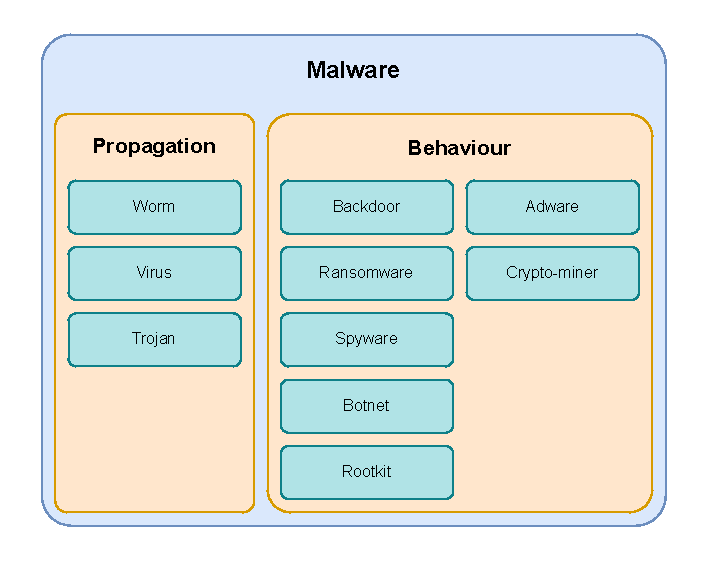
\includegraphics[width=0.7\textwidth]{../assets/malware-taxonomy.pdf}
    \caption{Categories of Malware, including both the means of propagation and behaviour on an infected host.}
    \label{fig:malware-taxonomy}
\end{figure}

As outlined in the previous section, malware are a form of software that have a detrimental impact on the expected operation of an infected system. However, both this definition, and formal definitions, such as the one presented by~\citep{kramerGeneralDefinitionMalware2010a}, fail to define what is meant by harmful. Therefore, we define harmful behaviour as actions that are in violation of the Confidentiality-Integrity-Availability (CIA) triad~\citep{cochranCIATriadSafeguarding2024}. This is a principle used to guide security policies that outline the need for a system to be protected against unauthorised access (Confidentiality), modification (integrity), and reliable (availability) to be considered secure. 

Malware can be categorised based on its behaviour, and its method of propagation. We present the following taxonomy based on the work of~\cite{manirihoSystematicLiteratureReview2024} shown in~\autoref{fig:malware-taxonomy} that outlines the different kinds of malware seen by security researchers, and how they are spread. Note that categories within this taxonomy are not mutually exclusive, as they often belong to multiple categories at once. 

\begin{itemize}
    \item \textbf{Worm} | Malicious software that automatically propagates throughout a network. 
    \item \textbf{Virus} | Programs that modify other programs to replicate themselves throughout an infected host. 
    \item \textbf{Trojans} | Malware that disguises itself as a legitimate program to infect a host.
    \item \textbf{Backdoor} | Malware that provides covert remote access to infected systems. 
    \item \textbf{Ransomware} | Malware that denies access to systems or information until a fee is paid.
    \item \textbf{Spyware} | Malware that spy on the user without their knowledge, often extracting information such as credentials, keyboard logs, and live screenshots of the user's activity. 
    \item \textbf{Botnet} | Malware that integrate infected systems into a coordinated network of agents. 
    \item \textbf{Rootkit} | Malware providing privileged access to an infected system.
    \item \textbf{Adware} | Malware that display advertisements on the host machine.
    \item \textbf{Crypto-miner} | Malware that hijack the user's hardware to mine cryptocurrencies.
\end{itemize}

\subsection{Evasion Techniques}

The earliest forms of malware detection used a combination of unique signatures associated with malicious programs, and a set of heuristics to identify malicious programs~\citep{a.saeedSurveyMalwareMalware2013}. In response to this, developers of malicious software began using evasion techniques that aim to decieve these systems. This was done in order to maximise the amount of potential damage the software is able to do to an infected host before it is identified and removed. These evasion techniques include obfuscation, environmental awareness, and living-off-the-land. In the following section, we discuss these techniques, and why they are effective at defeating existing malware detection. 

\subsubsection{Obfuscation}

\begin{figure}
    \centering 
    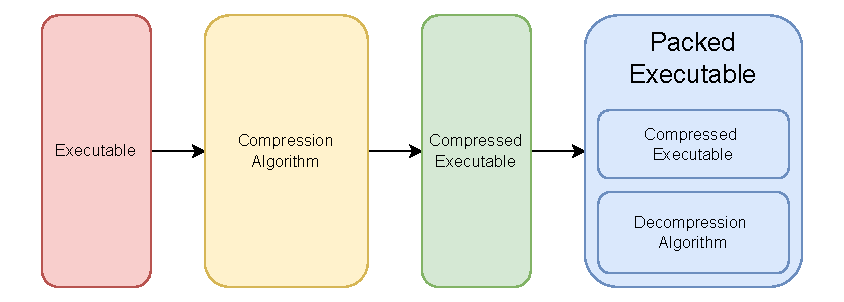
\includegraphics[width=0.7\textwidth]{../assets/binary-packing.pdf}
    \caption{How binary packing can be used to reduce the size of an executable program, and obscure its behaviour.}
    \label{fig:binary-packing}
\end{figure}

Obfuscation is defined as the act of making something more challenging to understand. In the context of malware, it relates to techniques that alter the syntactic structure of a program, while maintaining its original behavioural characteristics. In this section, we explore different forms of obfuscation, and their effectiveness in evading detection. 

Register re-assignment is the process of randomly reallocating registers used by the program~\citep{balakrishnanCodeObfuscationLiterature2005}. Registers are small areas of memory within the CPU that store information used during the program's execution. By changing which registers are used to store information, the physical structure of the program is changed, while maintaining its behavior. This defeats simple malware detection solutions that use the unique cryptographic hashes of a program as its signature. 

Dead code insertion is simple form of obfuscation that inserts instructions which have no impact on the state of the program's execution. These instructions include the no-operation (\texttt{nop}), swapping the value stored in a register with itself, and adding zero to a register to name a few. This again modifies the physical structure of a program, without impacting its behaviour. This is not limited to singular instructions, and can include the insertion of functions which are never executed which can make the program more challenging to identify. However, dead code is relatively easy to identify and remove.

Code transposition modifies the order of code the program~\citep{christodorescuStaticAnalysisExecutables2004} to obscure its signatures by moving small units of code known as basic blocks. These basic blocks do not contain jumps, such as loops or conditional statements. To ensure the program behaves as expected, all references to the relocated basic blocks are updated with its new location. This evades detection in a similar way to the obfuscation techniques discussed previously, by creating unique representations of the same program that give produce different signatures not recognised by the analysis software. 

Despite the ability of these techniques to trick early anti-malware approaches, more sophisticated approaches are more resiliant to these forms of obfuscation. These approaches use an intermediate representation of the program, that normalise the structure of a program resulting in a representation that is indentical to the un-obfuscated representation. To evade these solutions, more sophisticated forms of obfuscation are needed. One such example of this is known as binary packing, where the malicious portion of code is encoded and stored as data within another program that decoded and executes the payload. Encoding can take many forms, such as encrpytion or compression, but they typically make it challenging to retrieve the decoded payload without running the program. However, the portion of the packed binary responsible for decoding and execution will often remain constant, meaning it can be used for identification. Some malware developers employ the aforementioned obfuscation techniques to obscure the decoder and avoid detection. This is known as Oligomorphic and Polymorphic malware~\citep{youMalwareObfuscationTechniques2010}. 

\subsubsection{Environmental Awareness}

As a result of the previously discussed obfuscation techniques, relying on the static structure of a program may be insufficient to reliably detect malware. It is for this reason that dynamic features are considered to be more robust indicators of malicious programs, as the behaviour of a program is invariant to obfuscation. These dynamic features are observed at execution time and can include sequences of system API calls, modifications to the filesystem and system configuration, and internet traffic. However, this requires running a potentially malicious program, which could have harmful effects on the host system. It is for this reason that execution of a potentially malicious program occurs within a sandbox, an environment where the harmful actions can occur with no implications on the security of the system. This sandbox is typically a virtual machine or a containerized application, that's representative of the software's intended target. 

To obscure the behaviour of the program, the developers of these malicious programs will attempt to check if the program is running within a virtual machine. Common heuristics used by malicious programs include system hardware characteristics (CPU core count, RAM size, etc), the presence of shared libraries used to communicate between the sandbox and its host, and the number of processes running on the potential host. If the program determines that it is likely to be running within a sandbox, it will refuse to execute the malicious portion of the code, and exit early. This prevents the observer from gaining any information about its behavioural characteristics, preventing the creation of dynamic malicious signatures. 

\subsubsection{Living-off-the-land}

In recent years, the sophistication of malware has increased dramatically. Living off the land refers to an evasion technique used by advanced malware that significantly reduces the ability of existing security solutions to detect the presence of malware on a host system. 

Upon gaining access to a system, often through software vulnerabilities, or social engineering, the malicious software will make use of trusted programs already present to further compromise the host. For example, certain tools in windows machines can make changes to the system registry, which is a trusted location that isn't typically analysed by anti-malware software. It remains consistent between system restarts, and includes a list of programs that should always be executed upon turning on. This allows a threat actor to install malicious software within a trusted location, that is persistent between restarts, that is not saved to the host's disk. This is known as fileless malware. 

As the malware does not exist on disk, it is extremely difficult to detect by conventional means. Furthermore, as they rely on the functionality of trusted system programs, which are highly likely to be present on all targets. 

\section{Related Work}


Malware detection is a challenging problem, and many approaches have been proposed since the first forms of malicious software were seen in the 1980s. The earliest form of malware detection used a database containing the unique signatures of malicious programs. While similar signature based approaches are still in use today, there is much interest in advanced methods, that are robust to evasion techniques, and that able to identify novel forms of malware~\citep{m.ComprehensiveSurveyDeep2023,merabetSurveyMalwareDetection2019,aboaojaMalwareDetectionIssues2022,idikamathurSurveyMalwareDetection2007}. These advanced techniques employ a wide variety of technologies, such as multiple sequence alignment of API call sequences~\citep{kiNovelApproachDetect2015}, machine learning~\citep{kambojDetectionMalwareDownloaded2023}, and deep learning.

These techniques typically fall into one of two categories, based on how the features used to classify programs are extracted which are as follows. 

\begin{itemize}
    \item \textbf{Static} | Features extracted from the structure of a program
    \item \textbf{Dynamic} | Features extracted during the execution of the program
\end{itemize}

Static approaches use features extracted from the contents of an executable, and do not require executing the program. Common features used to identify malware include greyscale images of the executable~\citep{niMalwareIdentificationUsing2018,jainConvolutionalNeuralNetworks2020,habibiPerformanceEvaluationCNN2023}, printable strings~\citep{tianAutomatedClassificationSystem2009,singhDetectionMaliciousSoftware2020,schultzDataMiningMethods2001a}, and sequences of instructions~\citep{kakisimSequentialOpcodeEmbeddingbased2022,wangDeepLearningRegularization2021,daremVisualizationDeeplearningbasedMalware2021}. 

In~\cite{schultzDataMiningMethods2001a}, the authors use static features such as printable ASCII strings to train various machine learning classifiers to detect malware. In their experiments, they found that the Naive Bayes algorithm was best suited to the problem, achieving 97\% classification accuracy. This is one of the first papers that introduce the usage of machine learning in this domain, and the high accuracy of their experiment shows its potential over conventional signature or heuristic methods. However, the dataset used in this work was small, and featured an unbalanced class distribution of 3265 malicious programs, and only 1001 benign which would likely have an adverse effect on the generalisability of their proposed models. Furthermore, malware often obfuscate strings that are decoded during execution, which would be sufficient to defeat their proposed approach. 

Much of the literature relating to static malware detection use convolutional neural networks to distinguish between malicious and benign programs~\citep{niMalwareIdentificationUsing2018,jainConvolutionalNeuralNetworks2020,habibiPerformanceEvaluationCNN2023}. In~\cite{aslanNewMalwareClassification2021}, the authors represent an executable as a greyscale image, and train a convolutional neural network (CNN) to detect malware. While their proposed approach is able to effectively distinguish between executable classes, CNNs require constant input size. Therefore, resizing of the image representation is necessary. Malicious programs are often smaller than benign programs, meaning that in datasets where there is significant variation in size between classes, compression artifacts may be more prevalant in once class, leading to the model developing an insufficient solution. In~\cite{sharmaMalwareDetectionUsing2019}, the authors also use a CNN to detect malware. Instead of using a 2-dimensional CNN however, the authors opt to use a 1-dimensional variant. This led to better performance than other CNN based approaches, as the vertical spatial dependence, which is largely irrelevant in malware detection, is removed. However, it still has the same requirement as the previously discussed approach. 

Instruction sequences have also been explored as static features in malware detection. For example, in~\citep{attaluriProfileHiddenMarkov2009,runwalOpcodeGraphSimilarity2012}, the authors utilise hidden markov models and achieve promising results. As these models consider what actions are being performed by the host system without having to execute the program, they offer a solution that we believe to be more resilient to obfuscation than other static approaches. 

Extending upon the idea of utilising instruction sequences for malware detection,~\citep{demirciStaticMalwareDetection2022} outline an approach in which they propose the use of stacked bidirectional Long-Short Term Memory (BiLSTM) and pre-trained language models including BERT~\citep{devlinBERTPretrainingDeep2019a}, and GPT-2~\citep{radfordLanguageModelsArea}. In their investigation, the BiLSTM model was able to achieve 98\% classification accuracy whereas the pre-trained transformer models achieved only 77\%. Transformer models have been shown to be a powerful technique for sequence classification problems, and as such, this result is surprising. We believe this to be a result of the corpora used to pre-train the transformer models used in their investigation, which are comprised of mostly english texts. The understanding of these models would thus be limited to languages similar to english, and may struggle to understand the intricacies of assembly language, impacting their ability to reliably classify malware. 

Previous research has also established the use of pre-trained language models in malware detection on the metadata of an executable. In~\cite{rahaliMalBERTMalwareDetection2021}, the authors fine-tune BERT on text gathered from the manifest file found in android applications. This file contains information pertaining to the activities, background tasks, event listeners, and permissions granted to an application. Their model was able to achieve 97\% binary classification accuracy, in comparison to~\citep{demirciStaticMalwareDetection2022} which was only able to achieve 77\% with the same model, trained on instruction sequences. We believe this discrepancy to be a result of the language found in these manifest files being more closely related to the pre-training corpora of the BERT model. This would enable their model to better understand the information found in the manifest, and its use in distinguishing between benign and malicious executables. Their approach however, is limited to environments where a file containing metadata are required, such as mobile operating systems, making it unsuitable for desktop malware detection. 

The performance of static malware detection approaches vary, depending on the detection method used, the availability of data, and other factors, but it is well established that they are particularly vulnerable to obfuscation. In~\cite{bacciImpactCodeObfuscation2018}, the authors investigate the impact of obfuscation on the performance of static and dynamic malware detectors on android devices. They found that while dynamic methods are not significantly impacted by the presence of obfuscation, static techniques are more affected. However, by training static methods on obfuscated programs, it is possible to mitigate this problem to some extent. 

Furthermore, dynamic methods generally tend to be more capable than static methods~\citep{damodaranComparisonStaticDynamic2017}. This is somewhat to be expected, as behaviour is more indicative of malicious actions, especially when obfuscation is used to hide a program's intent. However, dynamic methods require a sandbox to execute a program for analysis, without causing damage to a host. This typically takes the form of a remote, virtual machine as running such a sandbox locally would have a significant computational cost. As a result of this, dynamic methods require both significant compute resources, and an internet connection, which is not guaranteed. It is for this reason that static methods, that can identify potentially malicious programs, without an internet connection is needed for enhanced protection from this threat. 

In addition to the high resource requirements associated with dynamic feature extraction, sophisticated evasion techniques such as environmental awareness and living off the land provide malware developers with the capabilities to obscure the dynamic features. For example, by either preventing execution within virtual machines, or using trusted binaries already located on a host system. Furthermore, novel obfuscation techniques, such as the one proposed by~\cite{liAPIASONovelAPI2023}, is able to obscure which system API calls are made by a program. This is a widely used dynamic feature for detecting malware, and the proposed technique enables the malware to call these system APIs without triggering system hooks used to track which methods are called during a program's execution. Therefore, despite offering better performance than static methods, dynamic methods are also vulnerable to evasion techniques.

\section{Future Research Directions}

Our analysis of the literature relating to this field, we have found that there are a number of promising areas of investigation. Static approaches, while less robust to structural obfuscation, are less resource intensive and are able to be run locally. Dynamic features offer better performance than its static counterpart, yet are still vulnerable to advanced evasion techniques that may render them less effective than static. Furthermore, the requirements associated with dynamic feature extraction are a significant barrier to their deployment, and demonstrate the need for efficient and effective static methods for detecting malware. 

We propose investigating a transformer model, that firstly learns the semantics of assembly language, then fine-tuned on a downstream sequence classification problem. While transformers can be expensive to run locally, we believe that the simple nature of the language will allow us to create a less complex model that is able to reliably and accurately identify malware.

\end{document}